\documentclass[1p]{elsarticle_modified}
%\bibliographystyle{elsarticle-num}

%\usepackage[colorlinks]{hyperref}
%\usepackage{abbrmath_seonhwa} %\Abb, \Ascr, \Acal ,\Abf, \Afrak
\usepackage{amsfonts}
\usepackage{amssymb}
\usepackage{amsmath}
\usepackage{amsthm}
\usepackage{scalefnt}
\usepackage{amsbsy}
\usepackage{kotex}
\usepackage{caption}
\usepackage{subfig}
\usepackage{color}
\usepackage{graphicx}
\usepackage{xcolor} %% white, black, red, green, blue, cyan, magenta, yellow
\usepackage{float}
\usepackage{setspace}
\usepackage{hyperref}

\usepackage{tikz}
\usetikzlibrary{arrows}

\usepackage{multirow}
\usepackage{array} % fixed length table
\usepackage{hhline}

%%%%%%%%%%%%%%%%%%%%%
\makeatletter
\renewcommand*\env@matrix[1][\arraystretch]{%
	\edef\arraystretch{#1}%
	\hskip -\arraycolsep
	\let\@ifnextchar\new@ifnextchar
	\array{*\c@MaxMatrixCols c}}
\makeatother %https://tex.stackexchange.com/questions/14071/how-can-i-increase-the-line-spacing-in-a-matrix
%%%%%%%%%%%%%%%

\usepackage[normalem]{ulem}

\newcommand{\msout}[1]{\ifmmode\text{\sout{\ensuremath{#1}}}\else\sout{#1}\fi}
%SOURCE: \msout is \stkout macro in https://tex.stackexchange.com/questions/20609/strikeout-in-math-mode

\newcommand{\cancel}[1]{
	\ifmmode
	{\color{red}\msout{#1}}
	\else
	{\color{red}\sout{#1}}
	\fi
}

\newcommand{\add}[1]{
	{\color{blue}\uwave{#1}}
}

\newcommand{\replace}[2]{
	\ifmmode
	{\color{red}\msout{#1}}{\color{blue}\uwave{#2}}
	\else
	{\color{red}\sout{#1}}{\color{blue}\uwave{#2}}
	\fi
}

\newcommand{\Sol}{\mathcal{S}} %segment
\newcommand{\D}{D} %diagram
\newcommand{\A}{\mathcal{A}} %arc


%%%%%%%%%%%%%%%%%%%%%%%%%%%%%5 test

\def\sl{\operatorname{\textup{SL}}(2,\Cbb)}
\def\psl{\operatorname{\textup{PSL}}(2,\Cbb)}
\def\quan{\mkern 1mu \triangleright \mkern 1mu}

\theoremstyle{definition}
\newtheorem{thm}{Theorem}[section]
\newtheorem{prop}[thm]{Proposition}
\newtheorem{lem}[thm]{Lemma}
\newtheorem{ques}[thm]{Question}
\newtheorem{cor}[thm]{Corollary}
\newtheorem{defn}[thm]{Definition}
\newtheorem{exam}[thm]{Example}
\newtheorem{rmk}[thm]{Remark}
\newtheorem{alg}[thm]{Algorithm}

\newcommand{\I}{\sqrt{-1}}
\begin{document}

%\begin{frontmatter}
%
%\title{Boundary parabolic representations of knots up to 8 crossings}
%
%%% Group authors per affiliation:
%\author{Yunhi Cho} 
%\address{Department of Mathematics, University of Seoul, Seoul, Korea}
%\ead{yhcho@uos.ac.kr}
%
%
%\author{Seonhwa Kim} %\fnref{s_kim}}
%\address{Center for Geometry and Physics, Institute for Basic Science, Pohang, 37673, Korea}
%\ead{ryeona17@ibs.re.kr}
%
%\author{Hyuk Kim}
%\address{Department of Mathematical Sciences, Seoul National University, Seoul 08826, Korea}
%\ead{hyukkim@snu.ac.kr}
%
%\author{Seokbeom Yoon}
%\address{Department of Mathematical Sciences, Seoul National University, Seoul, 08826,  Korea}
%\ead{sbyoon15@snu.ac.kr}
%
%\begin{abstract}
%We find all boundary parabolic representation of knots up to 8 crossings.
%
%\end{abstract}
%\begin{keyword}
%    \MSC[2010] 57M25 
%\end{keyword}
%
%\end{frontmatter}

%\linenumbers
%\tableofcontents
%
\newcommand\colored[1]{\textcolor{white}{\rule[-0.35ex]{0.8em}{1.4ex}}\kern-0.8em\color{red} #1}%
%\newcommand\colored[1]{\textcolor{white}{ #1}\kern-2.17ex	\textcolor{white}{ #1}\kern-1.81ex	\textcolor{white}{ #1}\kern-2.15ex\color{red}#1	}

{\Large $\underline{12n_{0143}~(K12n_{0143})}$}

\setlength{\tabcolsep}{10pt}
\renewcommand{\arraystretch}{1.6}
\vspace{1cm}\begin{tabular}{m{100pt}>{\centering\arraybackslash}m{274pt}}
\multirow{5}{120pt}{
	\centering
	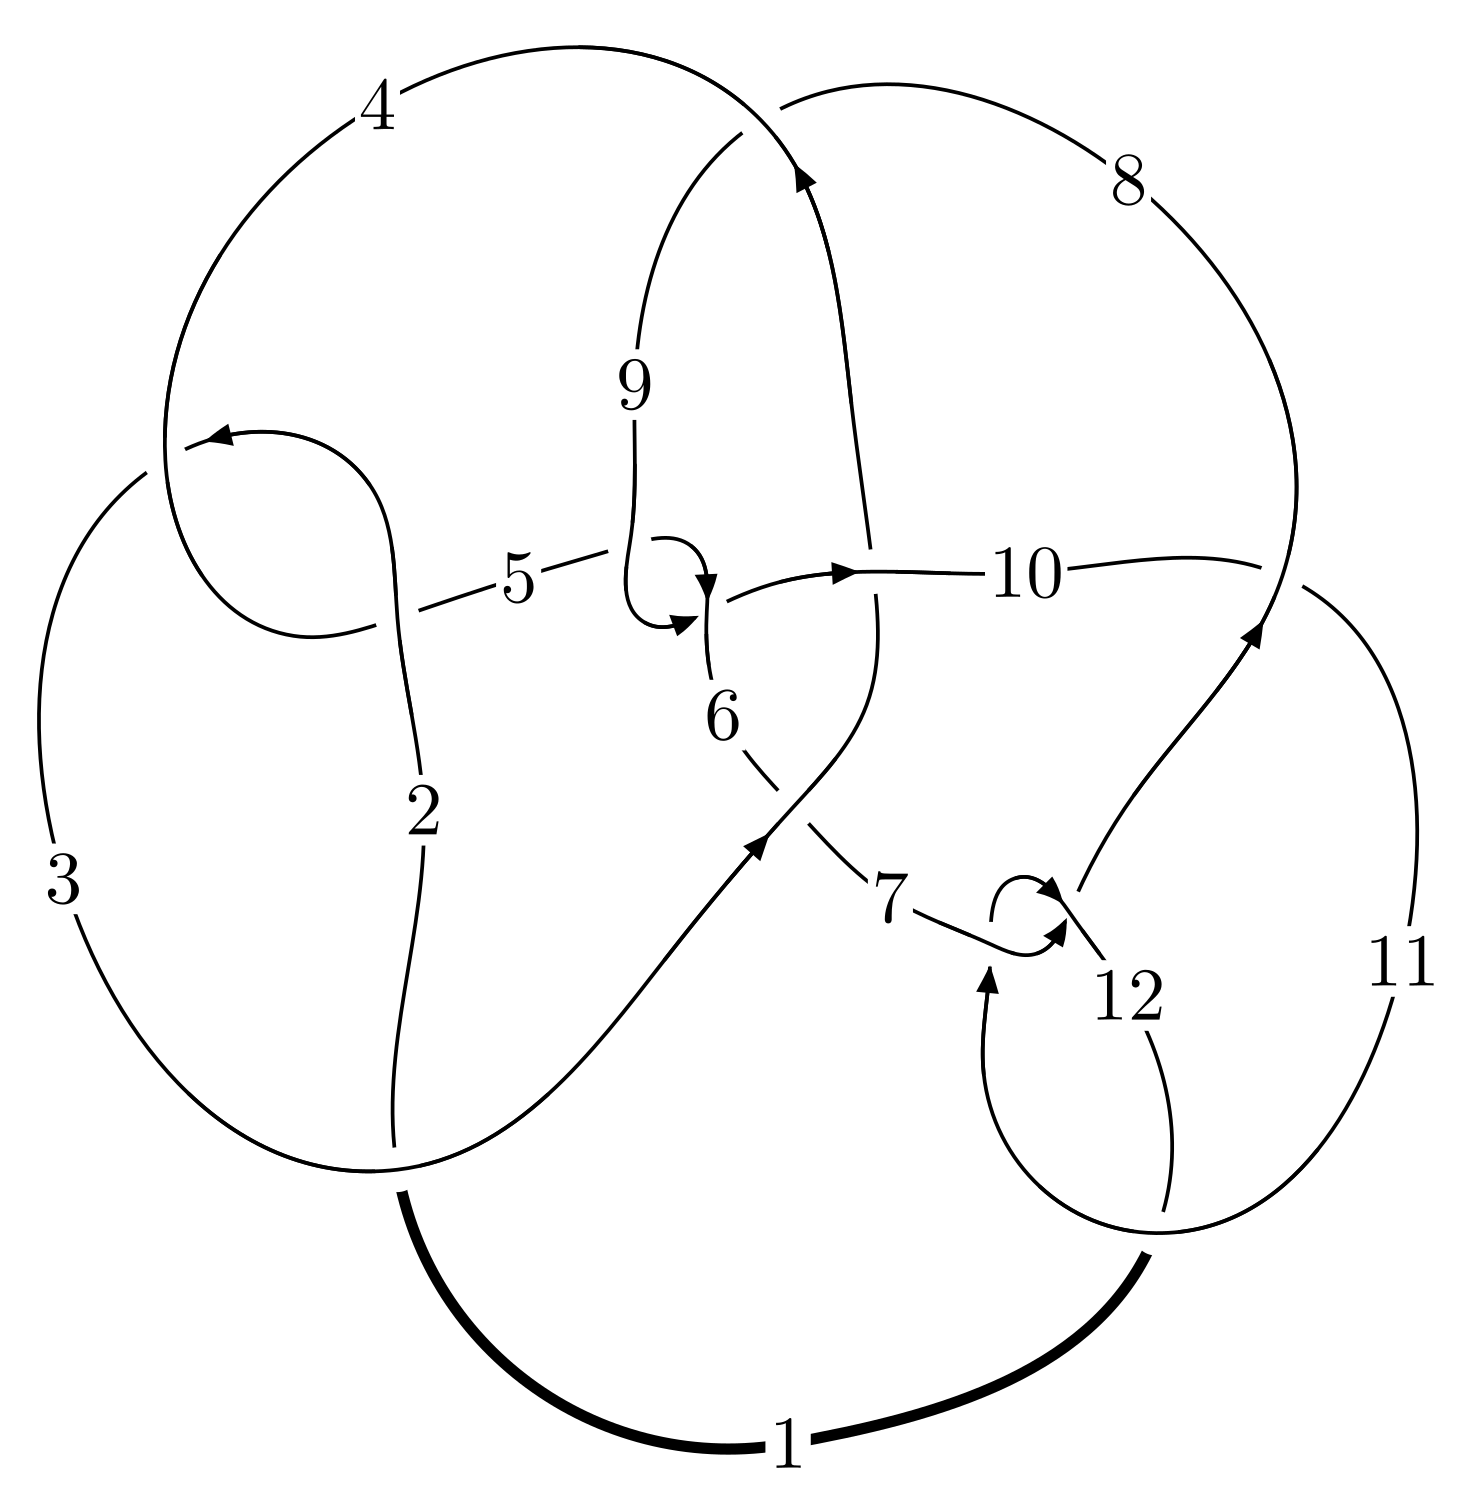
\includegraphics[width=112pt]{../../../GIT/diagram.site/Diagrams/png/2232_12n_0143.png}\\
\ \ \ A knot diagram\footnotemark}&
\allowdisplaybreaks
\textbf{Linearized knot diagam} \\
\cline{2-2}
 &
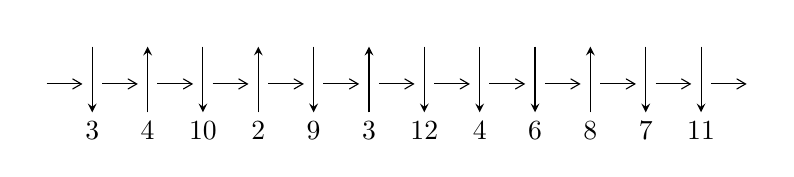
\begin{tikzpicture}[x=20pt, y=17pt]
	% nodes
	\node (C0) at (0, 0) {};
	\node (C1) at (1, 0) {};
	\node (C1U) at (1, +1) {};
	\node (C1D) at (1, -1) {3};

	\node (C2) at (2, 0) {};
	\node (C2U) at (2, +1) {};
	\node (C2D) at (2, -1) {4};

	\node (C3) at (3, 0) {};
	\node (C3U) at (3, +1) {};
	\node (C3D) at (3, -1) {10};

	\node (C4) at (4, 0) {};
	\node (C4U) at (4, +1) {};
	\node (C4D) at (4, -1) {2};

	\node (C5) at (5, 0) {};
	\node (C5U) at (5, +1) {};
	\node (C5D) at (5, -1) {9};

	\node (C6) at (6, 0) {};
	\node (C6U) at (6, +1) {};
	\node (C6D) at (6, -1) {3};

	\node (C7) at (7, 0) {};
	\node (C7U) at (7, +1) {};
	\node (C7D) at (7, -1) {12};

	\node (C8) at (8, 0) {};
	\node (C8U) at (8, +1) {};
	\node (C8D) at (8, -1) {4};

	\node (C9) at (9, 0) {};
	\node (C9U) at (9, +1) {};
	\node (C9D) at (9, -1) {6};

	\node (C10) at (10, 0) {};
	\node (C10U) at (10, +1) {};
	\node (C10D) at (10, -1) {8};

	\node (C11) at (11, 0) {};
	\node (C11U) at (11, +1) {};
	\node (C11D) at (11, -1) {7};

	\node (C12) at (12, 0) {};
	\node (C12U) at (12, +1) {};
	\node (C12D) at (12, -1) {11};
	\node (C13) at (13, 0) {};

	% arrows
	\draw[->,>={angle 60}]
	(C0) edge (C1) (C1) edge (C2) (C2) edge (C3) (C3) edge (C4) (C4) edge (C5) (C5) edge (C6) (C6) edge (C7) (C7) edge (C8) (C8) edge (C9) (C9) edge (C10) (C10) edge (C11) (C11) edge (C12) (C12) edge (C13) ;	\draw[->,>=stealth]
	(C1U) edge (C1D) (C2D) edge (C2U) (C3U) edge (C3D) (C4D) edge (C4U) (C5U) edge (C5D) (C6D) edge (C6U) (C7U) edge (C7D) (C8U) edge (C8D) (C9U) edge (C9D) (C10D) edge (C10U) (C11U) edge (C11D) (C12U) edge (C12D) ;
	\end{tikzpicture} \\
\hhline{~~} \\& 
\textbf{Solving Sequence} \\ \cline{2-2} 
 &
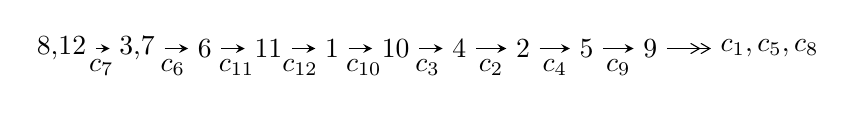
\begin{tikzpicture}[x=23pt, y=7pt]
	% node
	\node (A0) at (-1/8, 0) {8,12};
	\node (A1) at (17/16, 0) {3,7};
	\node (A2) at (17/8, 0) {6};
	\node (A3) at (25/8, 0) {11};
	\node (A4) at (33/8, 0) {1};
	\node (A5) at (41/8, 0) {10};
	\node (A6) at (49/8, 0) {4};
	\node (A7) at (57/8, 0) {2};
	\node (A8) at (65/8, 0) {5};
	\node (A9) at (73/8, 0) {9};
	\node (C1) at (1/2, -1) {$c_{7}$};
	\node (C2) at (13/8, -1) {$c_{6}$};
	\node (C3) at (21/8, -1) {$c_{11}$};
	\node (C4) at (29/8, -1) {$c_{12}$};
	\node (C5) at (37/8, -1) {$c_{10}$};
	\node (C6) at (45/8, -1) {$c_{3}$};
	\node (C7) at (53/8, -1) {$c_{2}$};
	\node (C8) at (61/8, -1) {$c_{4}$};
	\node (C9) at (69/8, -1) {$c_{9}$};
	\node (A10) at (11, 0) {$c_{1},c_{5},c_{8}$};

	% edge
	\draw[->,>=stealth]	
	(A0) edge (A1) (A1) edge (A2) (A2) edge (A3) (A3) edge (A4) (A4) edge (A5) (A5) edge (A6) (A6) edge (A7) (A7) edge (A8) (A8) edge (A9) ;
	\draw[->>,>={angle 60}]	
	(A9) edge (A10);
\end{tikzpicture} \\ 

\end{tabular} \\

\footnotetext{
The image of knot diagram is generated by the software ``\textbf{Draw programme}" developed by Andrew Bartholomew(\url{http://www.layer8.co.uk/maths/draw/index.htm\#Running-draw}), where we modified some parts for our purpose(\url{https://github.com/CATsTAILs/LinksPainter}).
}\phantom \\ \newline 
\centering \textbf{Ideals for irreducible components\footnotemark of $X_{\text{par}}$} 
 
\begin{align*}
I^u_{1}&=\langle 
-5018882 u^{19}-3159071 u^{18}+\cdots+35542844 b-8946208,\\
\phantom{I^u_{1}}&\phantom{= \langle  }4030002 u^{19}+3341564 u^{18}+\cdots+35542844 a+3081004,\;u^{20}- u^{19}+\cdots+4 u-4\rangle \\
I^u_{2}&=\langle 
-3 u^3 a+4 u^2 a-8 u^3+5 a u+2 u^2+13 b+2 a+9 u+1,\;3 u^3 a-2 u^2 a+2 a^2- u^2+4 a+6 u-2,\\
\phantom{I^u_{2}}&\phantom{= \langle  }u^4-2 u^2+2\rangle \\
\\
I^v_{1}&=\langle 
a,\;b+v,\;v^2- v+1\rangle \\
\end{align*}
\raggedright * 3 irreducible components of $\dim_{\mathbb{C}}=0$, with total 30 representations.\\
\footnotetext{All coefficients of polynomials are rational numbers. But the coefficients are sometimes approximated in decimal forms when there is not enough margin.}
\newpage
\renewcommand{\arraystretch}{1}
\centering \section*{I. $I^u_{1}= \langle -5.02\times10^{6} u^{19}-3.16\times10^{6} u^{18}+\cdots+3.55\times10^{7} b-8.95\times10^{6},\;4.03\times10^{6} u^{19}+3.34\times10^{6} u^{18}+\cdots+3.55\times10^{7} a+3.08\times10^{6},\;u^{20}- u^{19}+\cdots+4 u-4 \rangle$}
\flushleft \textbf{(i) Arc colorings}\\
\begin{tabular}{m{7pt} m{180pt} m{7pt} m{180pt} }
\flushright $a_{8}=$&$\begin{pmatrix}1\\0\end{pmatrix}$ \\
\flushright $a_{12}=$&$\begin{pmatrix}0\\u\end{pmatrix}$ \\
\flushright $a_{3}=$&$\begin{pmatrix}-0.113384 u^{19}-0.0940151 u^{18}+\cdots+0.649600 u-0.0866842\\0.141207 u^{19}+0.0888806 u^{18}+\cdots+0.434285 u+0.251702\end{pmatrix}$ \\
\flushright $a_{7}=$&$\begin{pmatrix}1\\- u^2\end{pmatrix}$ \\
\flushright $a_{6}=$&$\begin{pmatrix}0.334897 u^{19}-0.0768593 u^{18}+\cdots+0.470869 u+2.67956\\-0.0397535 u^{19}+0.166369 u^{18}+\cdots-0.371958 u-0.816791\end{pmatrix}$ \\
\flushright $a_{11}=$&$\begin{pmatrix}u\\- u^3+u\end{pmatrix}$ \\
\flushright $a_{1}=$&$\begin{pmatrix}- u^3\\u^5- u^3+u\end{pmatrix}$ \\
\flushright $a_{10}=$&$\begin{pmatrix}u^3\\- u^3+u\end{pmatrix}$ \\
\flushright $a_{4}=$&$\begin{pmatrix}-0.254108 u^{19}-0.153593 u^{18}+\cdots+0.947053 u-0.825468\\0.171597 u^{19}+0.0740954 u^{18}+\cdots+0.128017 u+0.521714\end{pmatrix}$ \\
\flushright $a_{2}=$&$\begin{pmatrix}-0.199337 u^{19}+0.0822480 u^{18}+\cdots+0.449295 u-0.850726\\0.0288459 u^{19}+0.0324049 u^{18}+\cdots+1.28582 u+0.0973546\end{pmatrix}$ \\
\flushright $a_{5}=$&$\begin{pmatrix}-0.0739774 u^{19}-0.140245 u^{18}+\cdots+0.662127 u-0.407213\\0.137706 u^{19}-0.0252866 u^{18}+\cdots+0.141019 u+0.447024\end{pmatrix}$ \\
\flushright $a_{9}=$&$\begin{pmatrix}-0.455718 u^{19}+0.276225 u^{18}+\cdots+0.309258 u-2.11593\\-0.200598 u^{19}-0.0655987 u^{18}+\cdots+0.985773 u-0.419904\end{pmatrix}$\\&\end{tabular}
\flushleft \textbf{(ii) Obstruction class $= -1$}\\~\\
\flushleft \textbf{(iii) Cusp Shapes $= -\frac{16163108}{8885711} u^{19}+\frac{7616138}{8885711} u^{18}+\cdots-\frac{81238406}{8885711} u-\frac{119525194}{8885711}$}\\~\\
\newpage\renewcommand{\arraystretch}{1}
\flushleft \textbf{(iv) u-Polynomials at the component}\newline \\
\begin{tabular}{m{50pt}|m{274pt}}
Crossings & \hspace{64pt}u-Polynomials at each crossing \\
\hline $$\begin{aligned}c_{1}\end{aligned}$$&$\begin{aligned}
&u^{20}+48 u^{19}+\cdots-52526 u+625
\end{aligned}$\\
\hline $$\begin{aligned}c_{2},c_{4}\end{aligned}$$&$\begin{aligned}
&u^{20}+24 u^{18}+\cdots+74 u+25
\end{aligned}$\\
\hline $$\begin{aligned}c_{3}\end{aligned}$$&$\begin{aligned}
&u^{20}+2 u^{19}+\cdots+12 u+5
\end{aligned}$\\
\hline $$\begin{aligned}c_{5},c_{9}\end{aligned}$$&$\begin{aligned}
&u^{20}+3 u^{19}+\cdots+u-1
\end{aligned}$\\
\hline $$\begin{aligned}c_{6}\end{aligned}$$&$\begin{aligned}
&u^{20}+4 u^{19}+\cdots-51528 u-13061
\end{aligned}$\\
\hline $$\begin{aligned}c_{7},c_{11}\end{aligned}$$&$\begin{aligned}
&u^{20}+u^{19}+\cdots-4 u-4
\end{aligned}$\\
\hline $$\begin{aligned}c_{8}\end{aligned}$$&$\begin{aligned}
&u^{20}-16 u^{19}+\cdots-18622 u-15107
\end{aligned}$\\
\hline $$\begin{aligned}c_{10}\end{aligned}$$&$\begin{aligned}
&u^{20}+3 u^{19}+\cdots+116 u+76
\end{aligned}$\\
\hline $$\begin{aligned}c_{12}\end{aligned}$$&$\begin{aligned}
&u^{20}+15 u^{19}+\cdots+80 u+16
\end{aligned}$\\
\hline
\end{tabular}\\~\\
\newpage\renewcommand{\arraystretch}{1}
\flushleft \textbf{(v) Riley Polynomials at the component}\newline \\
\begin{tabular}{m{50pt}|m{274pt}}
Crossings & \hspace{64pt}Riley Polynomials at each crossing \\
\hline $$\begin{aligned}c_{1}\end{aligned}$$&$\begin{aligned}
&y^{20}-400 y^{19}+\cdots-3308161926 y+390625
\end{aligned}$\\
\hline $$\begin{aligned}c_{2},c_{4}\end{aligned}$$&$\begin{aligned}
&y^{20}+48 y^{19}+\cdots-52526 y+625
\end{aligned}$\\
\hline $$\begin{aligned}c_{3}\end{aligned}$$&$\begin{aligned}
&y^{20}+24 y^{18}+\cdots-74 y+25
\end{aligned}$\\
\hline $$\begin{aligned}c_{5},c_{9}\end{aligned}$$&$\begin{aligned}
&y^{20}-45 y^{19}+\cdots+77 y+1
\end{aligned}$\\
\hline $$\begin{aligned}c_{6}\end{aligned}$$&$\begin{aligned}
&y^{20}+60 y^{19}+\cdots-809328142 y+170589721
\end{aligned}$\\
\hline $$\begin{aligned}c_{7},c_{11}\end{aligned}$$&$\begin{aligned}
&y^{20}-15 y^{19}+\cdots-80 y+16
\end{aligned}$\\
\hline $$\begin{aligned}c_{8}\end{aligned}$$&$\begin{aligned}
&y^{20}-120 y^{19}+\cdots-367173334 y+228221449
\end{aligned}$\\
\hline $$\begin{aligned}c_{10}\end{aligned}$$&$\begin{aligned}
&y^{20}+45 y^{19}+\cdots-68176 y+5776
\end{aligned}$\\
\hline $$\begin{aligned}c_{12}\end{aligned}$$&$\begin{aligned}
&y^{20}-15 y^{19}+\cdots+768 y+256
\end{aligned}$\\
\hline
\end{tabular}\\~\\
\newpage\flushleft \textbf{(vi) Complex Volumes and Cusp Shapes}
$$\begin{array}{c|c|c}  
\text{Solutions to }I^u_{1}& \I (\text{vol} + \sqrt{-1}CS) & \text{Cusp shape}\\
 \hline 
\begin{aligned}
u &= \phantom{-}1.027210 + 0.343771 I \\
a &= \phantom{-}0.25199 - 2.64585 I \\
b &= -0.766725 + 1.006540 I\end{aligned}
 & -2.86803 - 3.80264 I & -6.48723 + 4.67286 I \\ \hline\begin{aligned}
u &= \phantom{-}1.027210 - 0.343771 I \\
a &= \phantom{-}0.25199 + 2.64585 I \\
b &= -0.766725 - 1.006540 I\end{aligned}
 & -2.86803 + 3.80264 I & -6.48723 - 4.67286 I \\ \hline\begin{aligned}
u &= -1.095930 + 0.435073 I \\
a &= \phantom{-}1.163710 - 0.763492 I \\
b &= \phantom{-}0.458140 + 0.989102 I\end{aligned}
 & -2.45038 + 5.65982 I & -4.21302 - 7.24292 I \\ \hline\begin{aligned}
u &= -1.095930 - 0.435073 I \\
a &= \phantom{-}1.163710 + 0.763492 I \\
b &= \phantom{-}0.458140 - 0.989102 I\end{aligned}
 & -2.45038 - 5.65982 I & -4.21302 + 7.24292 I \\ \hline\begin{aligned}
u &= -0.722942 + 0.357669 I \\
a &= -0.128326 - 1.009150 I \\
b &= -0.238239 - 0.123051 I\end{aligned}
 & \phantom{-}0.99363 + 1.64776 I & \phantom{-}1.20276 - 5.62384 I \\ \hline\begin{aligned}
u &= -0.722942 - 0.357669 I \\
a &= -0.128326 + 1.009150 I \\
b &= -0.238239 + 0.123051 I\end{aligned}
 & \phantom{-}0.99363 - 1.64776 I & \phantom{-}1.20276 + 5.62384 I \\ \hline\begin{aligned}
u &= \phantom{-}0.106031 + 1.190120 I \\
a &= -0.299156 + 0.869186 I \\
b &= \phantom{-}0.09465 - 2.29475 I\end{aligned}
 & \phantom{-}19.2969 + 4.5215 I & -5.96688 - 1.69232 I \\ \hline\begin{aligned}
u &= \phantom{-}0.106031 - 1.190120 I \\
a &= -0.299156 - 0.869186 I \\
b &= \phantom{-}0.09465 + 2.29475 I\end{aligned}
 & \phantom{-}19.2969 - 4.5215 I & -5.96688 + 1.69232 I \\ \hline\begin{aligned}
u &= \phantom{-}0.634751 + 0.432509 I \\
a &= \phantom{-}0.196432 - 0.368569 I \\
b &= \phantom{-}0.643286 + 0.493353 I\end{aligned}
 & -1.74557 + 0.63892 I & -5.74453 + 1.51352 I \\ \hline\begin{aligned}
u &= \phantom{-}0.634751 - 0.432509 I \\
a &= \phantom{-}0.196432 + 0.368569 I \\
b &= \phantom{-}0.643286 - 0.493353 I\end{aligned}
 & -1.74557 - 0.63892 I & -5.74453 - 1.51352 I\\
 \hline 
 \end{array}$$\newpage$$\begin{array}{c|c|c}  
\text{Solutions to }I^u_{1}& \I (\text{vol} + \sqrt{-1}CS) & \text{Cusp shape}\\
 \hline 
\begin{aligned}
u &= \phantom{-}0.739383\phantom{ +0.000000I} \\
a &= -0.350220\phantom{ +0.000000I} \\
b &= \phantom{-}0.508808\phantom{ +0.000000I}\end{aligned}
 & -0.989681\phantom{ +0.000000I} & -10.9360\phantom{ +0.000000I} \\ \hline\begin{aligned}
u &= \phantom{-}1.350830 + 0.261047 I \\
a &= -1.05824 - 1.16450 I \\
b &= \phantom{-}0.045773 + 1.216250 I\end{aligned}
 & -4.75007 - 0.87462 I & -9.06700 + 0.37407 I \\ \hline\begin{aligned}
u &= \phantom{-}1.350830 - 0.261047 I \\
a &= -1.05824 + 1.16450 I \\
b &= \phantom{-}0.045773 - 1.216250 I\end{aligned}
 & -4.75007 + 0.87462 I & -9.06700 - 0.37407 I \\ \hline\begin{aligned}
u &= -0.255829 + 0.544433 I \\
a &= -0.156916 + 1.044260 I \\
b &= -0.341861 + 0.731952 I\end{aligned}
 & -0.11659 - 1.77179 I & -0.89537 + 3.37821 I \\ \hline\begin{aligned}
u &= -0.255829 - 0.544433 I \\
a &= -0.156916 - 1.044260 I \\
b &= -0.341861 - 0.731952 I\end{aligned}
 & -0.11659 + 1.77179 I & -0.89537 - 3.37821 I \\ \hline\begin{aligned}
u &= \phantom{-}1.35494 + 0.64126 I \\
a &= \phantom{-}1.91114 + 2.01731 I \\
b &= -0.21695 - 2.30777 I\end{aligned}
 & \phantom{-}15.4383 - 10.9552 I & -7.83113 + 4.63988 I \\ \hline\begin{aligned}
u &= \phantom{-}1.35494 - 0.64126 I \\
a &= \phantom{-}1.91114 - 2.01731 I \\
b &= -0.21695 + 2.30777 I\end{aligned}
 & \phantom{-}15.4383 + 10.9552 I & -7.83113 - 4.63988 I \\ \hline\begin{aligned}
u &= -1.52619\phantom{ +0.000000I} \\
a &= -1.06989\phantom{ +0.000000I} \\
b &= \phantom{-}0.168676\phantom{ +0.000000I}\end{aligned}
 & -9.28250\phantom{ +0.000000I} & -9.91420\phantom{ +0.000000I} \\ \hline\begin{aligned}
u &= -1.50565 + 0.55625 I \\
a &= -0.67058 + 2.22111 I \\
b &= -0.01682 - 2.17499 I\end{aligned}
 & \phantom{-}14.2365 + 1.7524 I & -8.57238 - 0.70411 I \\ \hline\begin{aligned}
u &= -1.50565 - 0.55625 I \\
a &= -0.67058 - 2.22111 I \\
b &= -0.01682 + 2.17499 I\end{aligned}
 & \phantom{-}14.2365 - 1.7524 I & -8.57238 + 0.70411 I\\
 \hline 
 \end{array}$$\newpage\newpage\renewcommand{\arraystretch}{1}
\centering \section*{II. $I^u_{2}= \langle -3 u^3 a-8 u^3+\cdots+2 a+1,\;3 u^3 a-2 u^2 a+2 a^2- u^2+4 a+6 u-2,\;u^4-2 u^2+2 \rangle$}
\flushleft \textbf{(i) Arc colorings}\\
\begin{tabular}{m{7pt} m{180pt} m{7pt} m{180pt} }
\flushright $a_{8}=$&$\begin{pmatrix}1\\0\end{pmatrix}$ \\
\flushright $a_{12}=$&$\begin{pmatrix}0\\u\end{pmatrix}$ \\
\flushright $a_{3}=$&$\begin{pmatrix}a\\0.230769 a u^{3}+0.615385 u^{3}+\cdots-0.153846 a-0.0769231\end{pmatrix}$ \\
\flushright $a_{7}=$&$\begin{pmatrix}1\\- u^2\end{pmatrix}$ \\
\flushright $a_{6}=$&$\begin{pmatrix}-1.61538 a u^{3}-1.80769 u^{3}+\cdots-0.923077 a+1.53846\\0.769231 a u^{3}+1.38462 u^{3}+\cdots+0.153846 a+1.07692\end{pmatrix}$ \\
\flushright $a_{11}=$&$\begin{pmatrix}u\\- u^3+u\end{pmatrix}$ \\
\flushright $a_{1}=$&$\begin{pmatrix}- u^3\\u^3- u\end{pmatrix}$ \\
\flushright $a_{10}=$&$\begin{pmatrix}u^3\\- u^3+u\end{pmatrix}$ \\
\flushright $a_{4}=$&$\begin{pmatrix}0.769231 a u^{3}+1.38462 u^{3}+\cdots+1.15385 a-0.923077\\-0.230769 a u^{3}-0.615385 u^{3}+\cdots+0.153846 a+0.0769231\end{pmatrix}$ \\
\flushright $a_{2}=$&$\begin{pmatrix}-0.384615 a u^{3}-2.19231 u^{3}+\cdots-0.0769231 a-1.53846\\0.461538 a u^{3}+2.23077 u^{3}+\cdots-0.307692 a+0.846154\end{pmatrix}$ \\
\flushright $a_{5}=$&$\begin{pmatrix}u^3\\- u^3+u\end{pmatrix}$ \\
\flushright $a_{9}=$&$\begin{pmatrix}1.61538 a u^{3}+2.80769 u^{3}+\cdots+0.923077 a-1.53846\\-0.769231 a u^{3}-2.38462 u^{3}+\cdots-0.153846 a-1.07692\end{pmatrix}$\\&\end{tabular}
\flushleft \textbf{(ii) Obstruction class $= 1$}\\~\\
\flushleft \textbf{(iii) Cusp Shapes $= -\frac{12}{13} u^3 a+\frac{16}{13} u^2 a+\frac{20}{13} u^3+\frac{20}{13} a u+\frac{60}{13} u^2+\frac{8}{13} a-\frac{16}{13} u-\frac{152}{13}$}\\~\\
\newpage\renewcommand{\arraystretch}{1}
\flushleft \textbf{(iv) u-Polynomials at the component}\newline \\
\begin{tabular}{m{50pt}|m{274pt}}
Crossings & \hspace{64pt}u-Polynomials at each crossing \\
\hline $$\begin{aligned}c_{1},c_{3},c_{4}\end{aligned}$$&$\begin{aligned}
&(u^2- u+1)^4
\end{aligned}$\\
\hline $$\begin{aligned}c_{2}\end{aligned}$$&$\begin{aligned}
&(u^2+u+1)^4
\end{aligned}$\\
\hline $$\begin{aligned}c_{5}\end{aligned}$$&$\begin{aligned}
&(u+1)^8
\end{aligned}$\\
\hline $$\begin{aligned}c_{6}\end{aligned}$$&$\begin{aligned}
&u^8+4 u^7+8 u^6+16 u^5+27 u^4+24 u^3+24 u^2+40 u+25
\end{aligned}$\\
\hline $$\begin{aligned}c_{7},c_{11}\end{aligned}$$&$\begin{aligned}
&(u^4-2 u^2+2)^2
\end{aligned}$\\
\hline $$\begin{aligned}c_{8}\end{aligned}$$&$\begin{aligned}
&u^8-4 u^7+8 u^6-16 u^5+27 u^4-24 u^3+24 u^2-40 u+25
\end{aligned}$\\
\hline $$\begin{aligned}c_{9}\end{aligned}$$&$\begin{aligned}
&(u-1)^8
\end{aligned}$\\
\hline $$\begin{aligned}c_{10}\end{aligned}$$&$\begin{aligned}
&(u^4+2 u^2+2)^2
\end{aligned}$\\
\hline $$\begin{aligned}c_{12}\end{aligned}$$&$\begin{aligned}
&(u^2+2 u+2)^4
\end{aligned}$\\
\hline
\end{tabular}\\~\\
\newpage\renewcommand{\arraystretch}{1}
\flushleft \textbf{(v) Riley Polynomials at the component}\newline \\
\begin{tabular}{m{50pt}|m{274pt}}
Crossings & \hspace{64pt}Riley Polynomials at each crossing \\
\hline $$\begin{aligned}c_{1},c_{2},c_{3}\\c_{4}\end{aligned}$$&$\begin{aligned}
&(y^2+y+1)^4
\end{aligned}$\\
\hline $$\begin{aligned}c_{5},c_{9}\end{aligned}$$&$\begin{aligned}
&(y-1)^8
\end{aligned}$\\
\hline $$\begin{aligned}c_{6},c_{8}\end{aligned}$$&$\begin{aligned}
&y^8-10 y^6+32 y^5+75 y^4-160 y^3+6 y^2-400 y+625
\end{aligned}$\\
\hline $$\begin{aligned}c_{7},c_{11}\end{aligned}$$&$\begin{aligned}
&(y^2-2 y+2)^4
\end{aligned}$\\
\hline $$\begin{aligned}c_{10}\end{aligned}$$&$\begin{aligned}
&(y^2+2 y+2)^4
\end{aligned}$\\
\hline $$\begin{aligned}c_{12}\end{aligned}$$&$\begin{aligned}
&(y^2+4)^4
\end{aligned}$\\
\hline
\end{tabular}\\~\\
\newpage\flushleft \textbf{(vi) Complex Volumes and Cusp Shapes}
$$\begin{array}{c|c|c}  
\text{Solutions to }I^u_{2}& \I (\text{vol} + \sqrt{-1}CS) & \text{Cusp shape}\\
 \hline 
\begin{aligned}
u &= \phantom{-}1.098680 + 0.455090 I \\
a &= -0.789474 + 0.479379 I \\
b &= \phantom{-}0.044910 + 0.232659 I\end{aligned}
 & -4.11234 - 5.69375 I & -10.00000 + 7.46410 I \\ \hline\begin{aligned}
u &= \phantom{-}1.098680 + 0.455090 I \\
a &= -1.17592 - 1.81004 I \\
b &= \phantom{-}0.04491 + 1.96471 I\end{aligned}
 & -4.11234 - 1.63398 I & -10.00000 + 0.53590 I \\ \hline\begin{aligned}
u &= \phantom{-}1.098680 - 0.455090 I \\
a &= -0.789474 - 0.479379 I \\
b &= \phantom{-}0.044910 - 0.232659 I\end{aligned}
 & -4.11234 + 5.69375 I & -10.00000 - 7.46410 I \\ \hline\begin{aligned}
u &= \phantom{-}1.098680 - 0.455090 I \\
a &= -1.17592 + 1.81004 I \\
b &= \phantom{-}0.04491 - 1.96471 I\end{aligned}
 & -4.11234 + 1.63398 I & -10.00000 - 0.53590 I \\ \hline\begin{aligned}
u &= -1.098680 + 0.455090 I \\
a &= -1.55613 - 1.07799 I \\
b &= \phantom{-}0.955090 + 0.232659 I\end{aligned}
 & -4.11234 + 1.63398 I & -10.00000 - 0.53590 I \\ \hline\begin{aligned}
u &= -1.098680 + 0.455090 I \\
a &= \phantom{-}1.52152 - 2.25267 I \\
b &= \phantom{-}0.95509 + 1.96471 I\end{aligned}
 & -4.11234 + 5.69375 I & -10.00000 - 7.46410 I \\ \hline\begin{aligned}
u &= -1.098680 - 0.455090 I \\
a &= -1.55613 + 1.07799 I \\
b &= \phantom{-}0.955090 - 0.232659 I\end{aligned}
 & -4.11234 - 1.63398 I & -10.00000 + 0.53590 I \\ \hline\begin{aligned}
u &= -1.098680 - 0.455090 I \\
a &= \phantom{-}1.52152 + 2.25267 I \\
b &= \phantom{-}0.95509 - 1.96471 I\end{aligned}
 & -4.11234 - 5.69375 I & -10.00000 + 7.46410 I\\
 \hline 
 \end{array}$$\newpage\newpage\renewcommand{\arraystretch}{1}
\centering \section*{III. $I^v_{1}= \langle a,\;b+v,\;v^2- v+1 \rangle$}
\flushleft \textbf{(i) Arc colorings}\\
\begin{tabular}{m{7pt} m{180pt} m{7pt} m{180pt} }
\flushright $a_{8}=$&$\begin{pmatrix}1\\0\end{pmatrix}$ \\
\flushright $a_{12}=$&$\begin{pmatrix}v\\0\end{pmatrix}$ \\
\flushright $a_{3}=$&$\begin{pmatrix}0\\- v\end{pmatrix}$ \\
\flushright $a_{7}=$&$\begin{pmatrix}1\\0\end{pmatrix}$ \\
\flushright $a_{6}=$&$\begin{pmatrix}1\\v-1\end{pmatrix}$ \\
\flushright $a_{11}=$&$\begin{pmatrix}v\\0\end{pmatrix}$ \\
\flushright $a_{1}=$&$\begin{pmatrix}v\\0\end{pmatrix}$ \\
\flushright $a_{10}=$&$\begin{pmatrix}v\\0\end{pmatrix}$ \\
\flushright $a_{4}=$&$\begin{pmatrix}-1\\- v\end{pmatrix}$ \\
\flushright $a_{2}=$&$\begin{pmatrix}v\\-1\end{pmatrix}$ \\
\flushright $a_{5}=$&$\begin{pmatrix}- v\\0\end{pmatrix}$ \\
\flushright $a_{9}=$&$\begin{pmatrix}v+1\\v-1\end{pmatrix}$\\&\end{tabular}
\flushleft \textbf{(ii) Obstruction class $= 1$}\\~\\
\flushleft \textbf{(iii) Cusp Shapes $= -4 v-4$}\\~\\
\newpage\renewcommand{\arraystretch}{1}
\flushleft \textbf{(iv) u-Polynomials at the component}\newline \\
\begin{tabular}{m{50pt}|m{274pt}}
Crossings & \hspace{64pt}u-Polynomials at each crossing \\
\hline $$\begin{aligned}c_{1},c_{4}\end{aligned}$$&$\begin{aligned}
&u^2- u+1
\end{aligned}$\\
\hline $$\begin{aligned}c_{2},c_{3},c_{6}\\c_{8}\end{aligned}$$&$\begin{aligned}
&u^2+u+1
\end{aligned}$\\
\hline $$\begin{aligned}c_{5}\end{aligned}$$&$\begin{aligned}
&(u-1)^2
\end{aligned}$\\
\hline $$\begin{aligned}c_{7},c_{10},c_{11}\\c_{12}\end{aligned}$$&$\begin{aligned}
&u^2
\end{aligned}$\\
\hline $$\begin{aligned}c_{9}\end{aligned}$$&$\begin{aligned}
&(u+1)^2
\end{aligned}$\\
\hline
\end{tabular}\\~\\
\newpage\renewcommand{\arraystretch}{1}
\flushleft \textbf{(v) Riley Polynomials at the component}\newline \\
\begin{tabular}{m{50pt}|m{274pt}}
Crossings & \hspace{64pt}Riley Polynomials at each crossing \\
\hline $$\begin{aligned}c_{1},c_{2},c_{3}\\c_{4},c_{6},c_{8}\end{aligned}$$&$\begin{aligned}
&y^2+y+1
\end{aligned}$\\
\hline $$\begin{aligned}c_{5},c_{9}\end{aligned}$$&$\begin{aligned}
&(y-1)^2
\end{aligned}$\\
\hline $$\begin{aligned}c_{7},c_{10},c_{11}\\c_{12}\end{aligned}$$&$\begin{aligned}
&y^2
\end{aligned}$\\
\hline
\end{tabular}\\~\\
\newpage\flushleft \textbf{(vi) Complex Volumes and Cusp Shapes}
$$\begin{array}{c|c|c}  
\text{Solutions to }I^v_{1}& \I (\text{vol} + \sqrt{-1}CS) & \text{Cusp shape}\\
 \hline 
\begin{aligned}
v &= \phantom{-}0.500000 + 0.866025 I \\
a &= \phantom{-0.000000 } 0 \\
b &= -0.500000 - 0.866025 I\end{aligned}
 & -1.64493 + 2.02988 I & -6.00000 - 3.46410 I \\ \hline\begin{aligned}
v &= \phantom{-}0.500000 - 0.866025 I \\
a &= \phantom{-0.000000 } 0 \\
b &= -0.500000 + 0.866025 I\end{aligned}
 & -1.64493 - 2.02988 I & -6.00000 + 3.46410 I\\
 \hline 
 \end{array}$$\newpage
\newpage\renewcommand{\arraystretch}{1}
\centering \section*{ IV. u-Polynomials}
\begin{tabular}{m{50pt}|m{274pt}}
Crossings & \hspace{64pt}u-Polynomials at each crossing \\
\hline $$\begin{aligned}c_{1}\end{aligned}$$&$\begin{aligned}
&((u^2- u+1)^5)(u^{20}+48 u^{19}+\cdots-52526 u+625)
\end{aligned}$\\
\hline $$\begin{aligned}c_{2}\end{aligned}$$&$\begin{aligned}
&((u^2+u+1)^5)(u^{20}+24 u^{18}+\cdots+74 u+25)
\end{aligned}$\\
\hline $$\begin{aligned}c_{3}\end{aligned}$$&$\begin{aligned}
&((u^2- u+1)^4)(u^2+u+1)(u^{20}+2 u^{19}+\cdots+12 u+5)
\end{aligned}$\\
\hline $$\begin{aligned}c_{4}\end{aligned}$$&$\begin{aligned}
&((u^2- u+1)^5)(u^{20}+24 u^{18}+\cdots+74 u+25)
\end{aligned}$\\
\hline $$\begin{aligned}c_{5}\end{aligned}$$&$\begin{aligned}
&((u-1)^2)(u+1)^8(u^{20}+3 u^{19}+\cdots+u-1)
\end{aligned}$\\
\hline $$\begin{aligned}c_{6}\end{aligned}$$&$\begin{aligned}
&(u^2+u+1)(u^8+4 u^7+\cdots+40 u+25)\\
&\cdot(u^{20}+4 u^{19}+\cdots-51528 u-13061)
\end{aligned}$\\
\hline $$\begin{aligned}c_{7},c_{11}\end{aligned}$$&$\begin{aligned}
&u^2(u^4-2 u^2+2)^2(u^{20}+u^{19}+\cdots-4 u-4)
\end{aligned}$\\
\hline $$\begin{aligned}c_{8}\end{aligned}$$&$\begin{aligned}
&(u^2+u+1)(u^8-4 u^7+\cdots-40 u+25)\\
&\cdot(u^{20}-16 u^{19}+\cdots-18622 u-15107)
\end{aligned}$\\
\hline $$\begin{aligned}c_{9}\end{aligned}$$&$\begin{aligned}
&((u-1)^8)(u+1)^2(u^{20}+3 u^{19}+\cdots+u-1)
\end{aligned}$\\
\hline $$\begin{aligned}c_{10}\end{aligned}$$&$\begin{aligned}
&u^2(u^4+2 u^2+2)^2(u^{20}+3 u^{19}+\cdots+116 u+76)
\end{aligned}$\\
\hline $$\begin{aligned}c_{12}\end{aligned}$$&$\begin{aligned}
&u^2(u^2+2 u+2)^4(u^{20}+15 u^{19}+\cdots+80 u+16)
\end{aligned}$\\
\hline
\end{tabular}\newpage\renewcommand{\arraystretch}{1}
\centering \section*{ V. Riley Polynomials}
\begin{tabular}{m{50pt}|m{274pt}}
Crossings & \hspace{64pt}Riley Polynomials at each crossing \\
\hline $$\begin{aligned}c_{1}\end{aligned}$$&$\begin{aligned}
&((y^2+y+1)^5)(y^{20}-400 y^{19}+\cdots-3.30816\times10^{9} y+390625)
\end{aligned}$\\
\hline $$\begin{aligned}c_{2},c_{4}\end{aligned}$$&$\begin{aligned}
&((y^2+y+1)^5)(y^{20}+48 y^{19}+\cdots-52526 y+625)
\end{aligned}$\\
\hline $$\begin{aligned}c_{3}\end{aligned}$$&$\begin{aligned}
&((y^2+y+1)^5)(y^{20}+24 y^{18}+\cdots-74 y+25)
\end{aligned}$\\
\hline $$\begin{aligned}c_{5},c_{9}\end{aligned}$$&$\begin{aligned}
&((y-1)^{10})(y^{20}-45 y^{19}+\cdots+77 y+1)
\end{aligned}$\\
\hline $$\begin{aligned}c_{6}\end{aligned}$$&$\begin{aligned}
&(y^2+y+1)(y^8-10 y^6+\cdots-400 y+625)\\
&\cdot(y^{20}+60 y^{19}+\cdots-809328142 y+170589721)
\end{aligned}$\\
\hline $$\begin{aligned}c_{7},c_{11}\end{aligned}$$&$\begin{aligned}
&y^2(y^2-2 y+2)^4(y^{20}-15 y^{19}+\cdots-80 y+16)
\end{aligned}$\\
\hline $$\begin{aligned}c_{8}\end{aligned}$$&$\begin{aligned}
&(y^2+y+1)(y^8-10 y^6+\cdots-400 y+625)\\
&\cdot(y^{20}-120 y^{19}+\cdots-367173334 y+228221449)
\end{aligned}$\\
\hline $$\begin{aligned}c_{10}\end{aligned}$$&$\begin{aligned}
&y^2(y^2+2 y+2)^4(y^{20}+45 y^{19}+\cdots-68176 y+5776)
\end{aligned}$\\
\hline $$\begin{aligned}c_{12}\end{aligned}$$&$\begin{aligned}
&y^2(y^2+4)^4(y^{20}-15 y^{19}+\cdots+768 y+256)
\end{aligned}$\\
\hline
\end{tabular}
\vskip 2pc
\end{document}